\begin{frame}[t, c]{}{}
  \begin{minipage}{.48\textwidth}
    \centering
    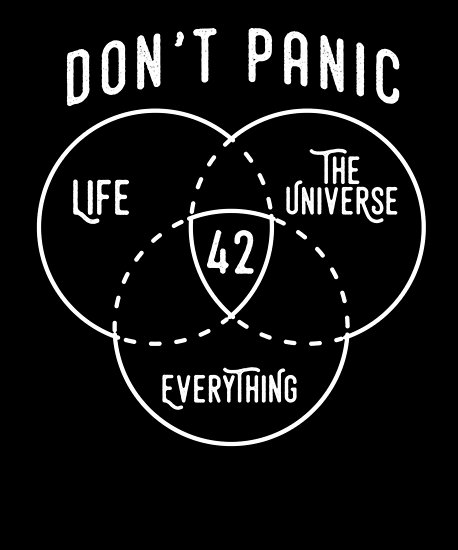
\includegraphics[width=.7\textwidth]{42}
  \end{minipage}%
  \hfill
  \begin{minipage}{.48\textwidth}
    \centering
    {
      \Large\textbf{Part IV}
    }
    
    \bigskip
    
    \rule{\textwidth}{0.001\textwidth}
    
    \bigskip
    
    {
      \large
      \textbf{Random thoughts on life, the universe and everything}
    }
    % \begin{itemize}
    % \item Summary
    % 
    % \medskip
    % 
    % \item Random thoughts and open problems.
    % \end{itemize}
    
  \end{minipage}
\end{frame}

\begin{frame}[t, c]{Random thoughts on life, the universe and everything}{Dimensionality reduction}
  \begin{minipage}{.68\textwidth}
    \begin{itemize}
    \item Dimensionality reduction as a preprocessing step to model the dynamics of physical systems has two competing objectives
      % 
      \begin{enumerate}
      \item Project the data in a low-dimensional latent space.
      \item The resulting coordinate system needs to be well-suited for modeling dynamics.
      \end{enumerate}
      
      \medskip
      
    \item While goal n\textsuperscript{o}1 can easily be formalized mathematically, goal n\textsuperscript{o}2 is more abstract.
    \end{itemize}
  \end{minipage}%
  \hfill
  \begin{minipage}{.28\textwidth}
    \centering
    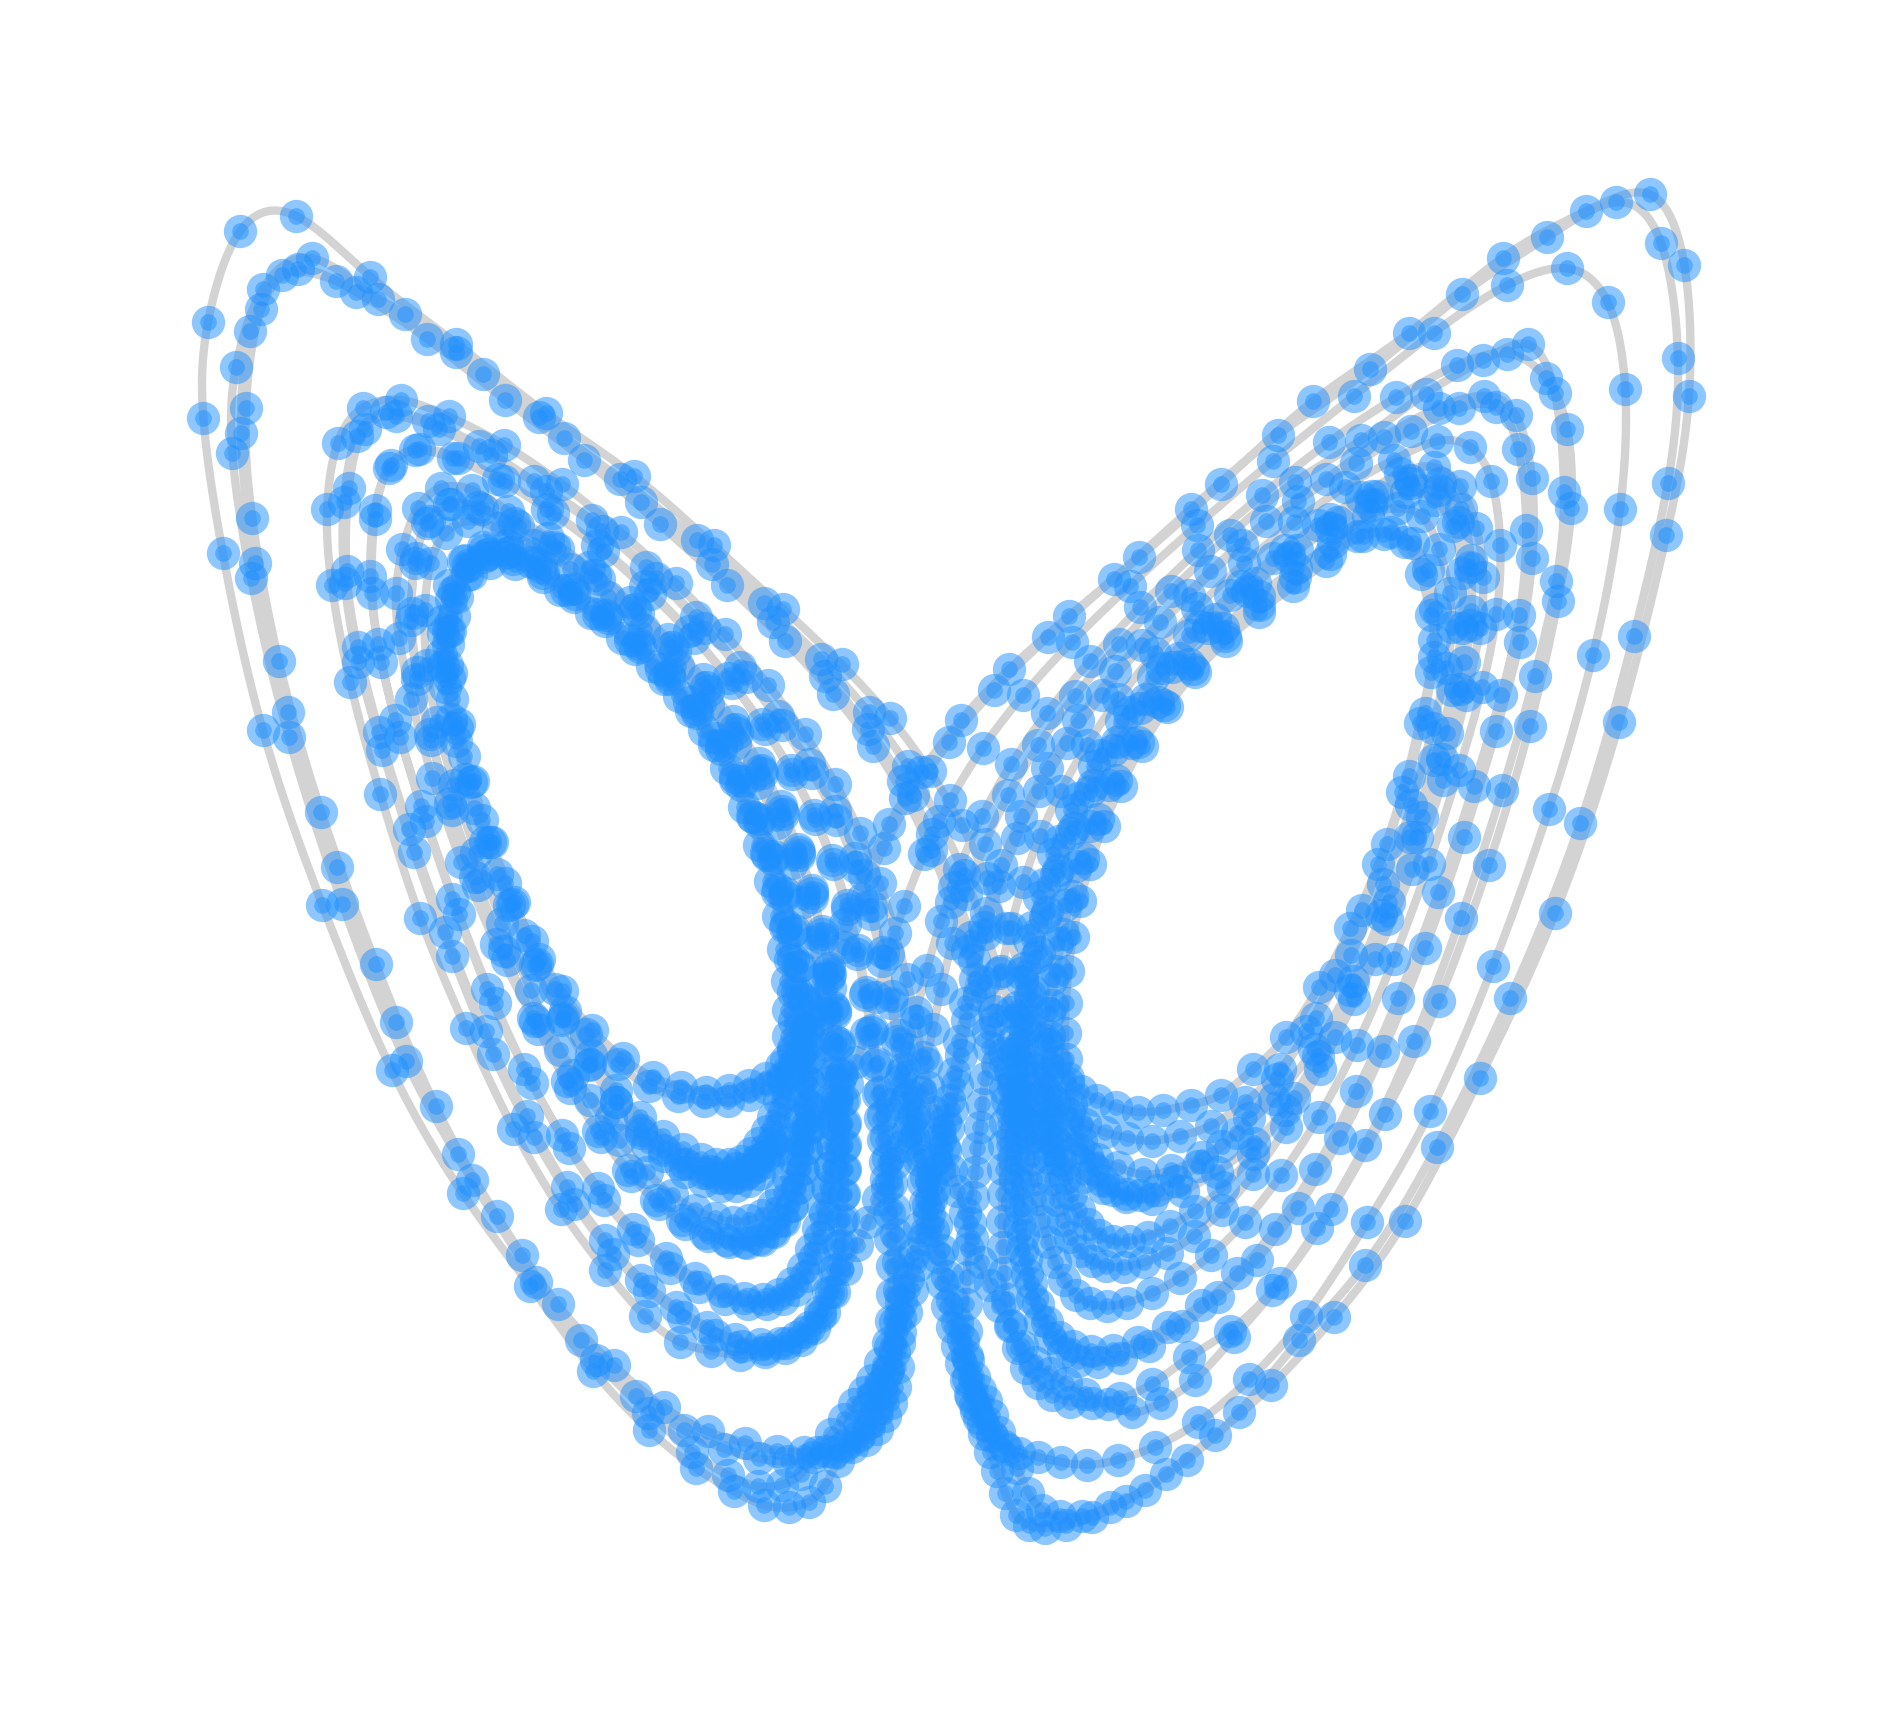
\includegraphics[width=\textwidth]{latent_space}
  \end{minipage}
  
  \vspace{1cm}
\end{frame}

\begin{frame}[t, c]{Random thought on life, the universe and everything}{Dimensionality reduction}
  \begin{minipage}{.68\textwidth}
    \begin{itemize}
    \item Given full-state data, personnal experience suggests that DMD-like techniques are well-suited.
      \begin{itemize}
      \item[\(	\hookrightarrow	\)] Relies on highly-efficient numerical linear algebra techniques.
      \item[\(	\hookrightarrow	\)] Inherently interpretable low-dimensional phase space.
      \end{itemize}
      
      \medskip
      
    \item From a dynamical system point of view, DMD has been related to the Koopman operator.
      \begin{itemize}
      \item[\(	\hookrightarrow	\)] Provides a coordinate system where the dynamics are approximately linear.
      \end{itemize}
    \end{itemize}
  \end{minipage}%
  \hfill
  \begin{minipage}{.28\textwidth}
    \centering
    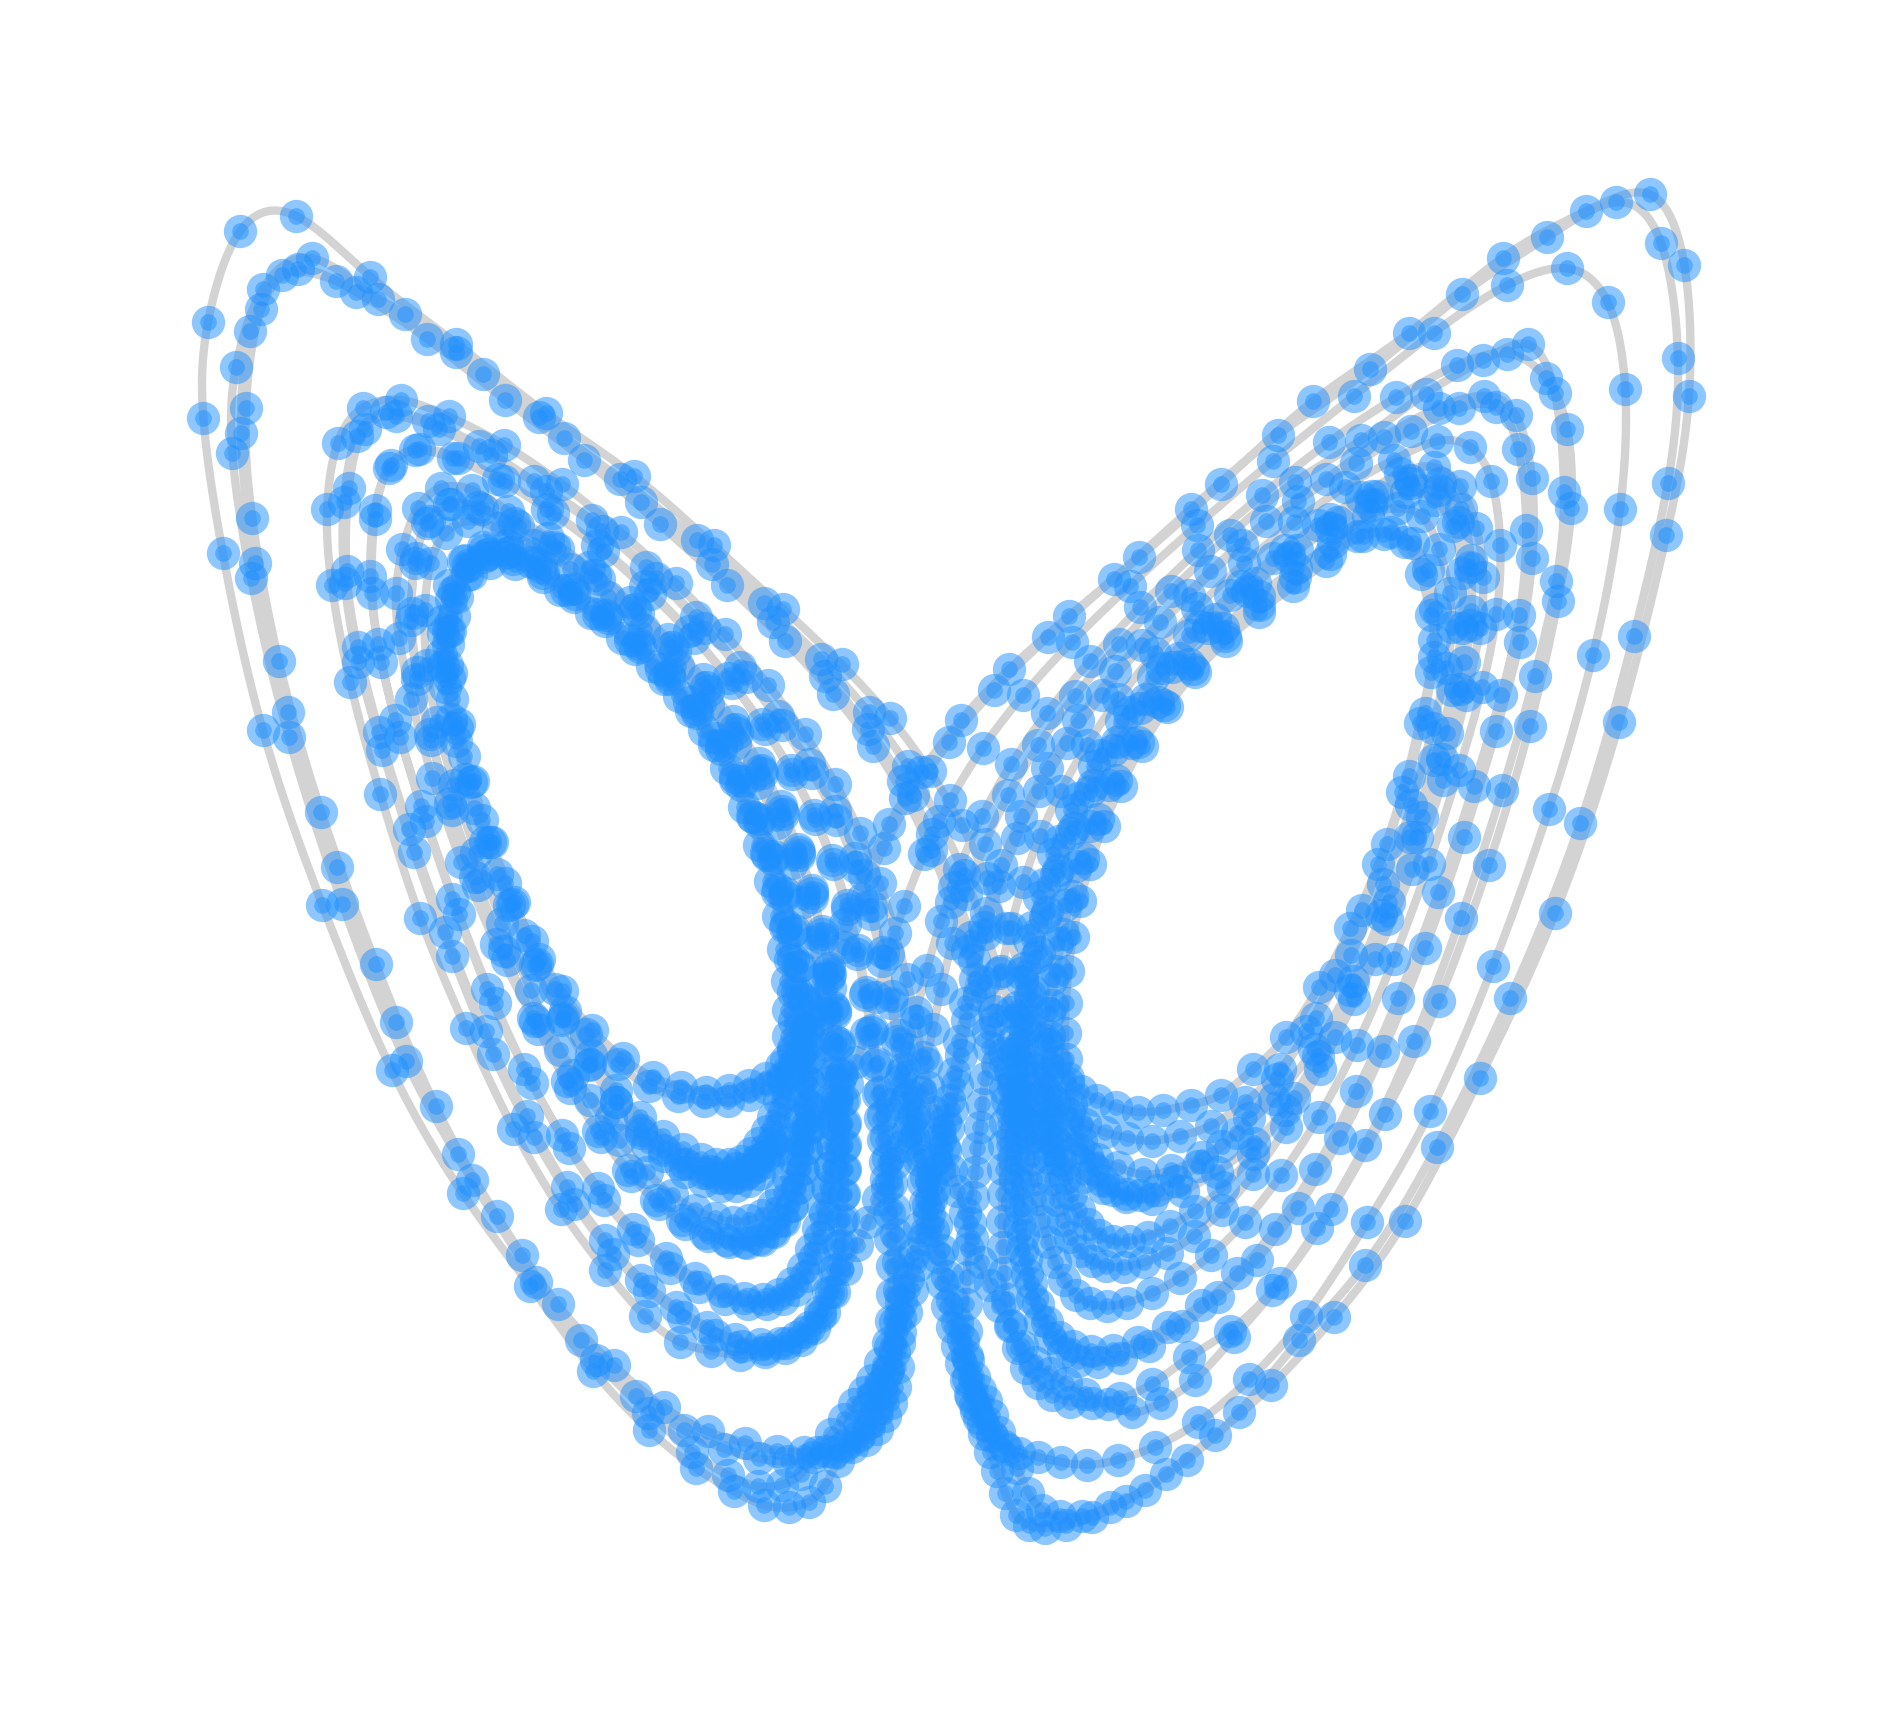
\includegraphics[width=\textwidth]{latent_space}
  \end{minipage}
  
  \vspace{1cm}
\end{frame}

\begin{frame}[t, c]{Random thoughts on life, the universe and everything}{Learning the dynamics}
  
  \begin{minipage}{.28\textwidth}
    \centering
    \Huge ?
  \end{minipage}%
  \hfill
  \begin{minipage}{.68\textwidth}
    \centering
    \begin{block}{}
      \centering
      \textbf{Learning the input-output map} \( \neq \) \textbf{Learning the physics}
    \end{block}
    
    \medskip
    
    \begin{itemize}
    \item Even on this ``simple'' example, basic ML algorithms are unable to learn the physical properties of the system.
      % \begin{itemize}
      % \item[\(	\hookrightarrow	\)] Any physical insights gained from the identified model may simply be wrong.
      % \end{itemize}
      
      \medskip
      
    \item Explicitely enforcing prior physical knowledge leads to easier training and orders of magnitude more accurate models.
      % \begin{itemize}
      % \item[\(	\hookrightarrow	\)] Correctly describes the physics and better generalization capabilities to non i.i.d.\ data.
      % \end{itemize}
    \end{itemize}
  \end{minipage}
  
  \vspace{1cm}
\end{frame}

\begin{frame}[t, c]{Random thoughts on life, the universe and everything}{How about scaling it up to realistic problems?}
  \centering
  \begin{block}
    \Large
    \centering
    \textbf{How to scale things up ?}
  \end{block}
  
  \bigskip
  
  \begin{itemize}
  \item[\(	\hookrightarrow	\)] \underline{Equivariant autoencoders} to encode existing spatial symmetries in the dimensionality reduction.
    
    \medskip
    
  \item[\(	\hookrightarrow	\)] Treating a neural network as a function \( \bm{f}(\bm{x}) \), use \underline{\(\partial\)ifferential programming} to apply differential operators (e.g.\ \( \nabla \cdot \bm{f}(\bm{x}) \), etc).
    
    \medskip
    
  \item[\(	\hookrightarrow	\)] Encode prior physical knowledge in the architecture / loss of the neural networks (see recent \emph{Lagrangian neural networks} for instance).
  \end{itemize}
  
  \vspace{1cm}
\end{frame}
